\PassOptionsToPackage{greek,english}{babel}
\documentclass{NSF_proposal_mod}
%PI: vardavas
%NSF ID: 000580367
%password:RedJupiter5
%Temp. Proposal #7091864
% Pin: 1234

% Pages to split the pdf at. 1,2,17,25,28,29,30



%\usepackage{epsfig}
%\documentclass[11pt]{article}

\usepackage[numbers,sort&compress]{natbib}


\usepackage[dvips]{graphicx}
\usepackage[table]{xcolor}
\usepackage{setspace}
\usepackage{enumitem}
\usepackage{adjustbox}
\usepackage{color}
\usepackage{boxedminipage}
\usepackage{amsfonts}
\usepackage{amsmath}
\usepackage{url}
\usepackage{caption}
\usepackage{tikz}
%\usepackage{setspace}
\usepackage{hyperref}
\usepackage{wrapfig}
\usepackage[T1]{fontenc}
\usepackage{tablefootnote}
\usepackage{multirow}
\usepackage{float} %After doing some more googling I came across the float package 
\restylefloat{table} %which lets you prevent LaTeX from repositioning the tables.
\usepackage[inline]{trackchanges} 
%\usepackage[margins]{trackchanges}
\addeditor{rv}
\addeditor{ap} 
\addeditor{kb} 
\addeditor{rl}
\addeditor{kk}
\addeditor{ga}
%%% Greek language
\usepackage[iso-8859-7]{inputenc}


%%% These lines of Question ID deal with breaking up long url links.
\makeatletter
\g@addto@macro{\UrlBreaks}{\UrlOrds}
\makeatother

% NSF proposal generation template style file.
% based on latex stylefiles  written by Stefan Llewellyn Smith and
% Sarah Gille, with contributions from other collaborators.

\newcommand{\jas}{{\it J. Atmos. Sci.}}
\newcommand{\jpo}{{\it J. Phys. Oceanogr.}}
\newcommand{\JPO}{{\it J. Phys. Oceanogr.}}
\newcommand{\jfm}{{\it J. Fluid Mech.}}
\newcommand{\jgr}{{\it J. Geophys. Res.}}
\newcommand{\JGR}{{\it J. Geophys. Res.}}
\newcommand{\jmr}{{\it J. Mar. Res.}}
\newcommand{\arfm}{{\it Ann. Rev. Fluid Mech.}}
\newcommand{\dsr}{{\it Deep-Sea Res.}}
\newcommand{\dao}{{\it Dyn. Atmos. Oceans}}
\newcommand{\jam}{{\it Journal of Applied Meteorology}}
\newcommand{\phfl}{{\it Phys. Fluids}}
\newcommand{\phfla}{{\it Phys. Fluids A}}
\newcommand{\PhilTrans}{{\it Philosophical Transactions of the Royal Society, 
London}}
\newcommand{\gafd}{{\it Geophys. Astrophys. Fluid Dyn.}}
\newcommand{\gfd}{{\it Geophys. Fluid Dyn.}}
\newcommand{\PCE}   {{\it Physics and Chemistry of the Earth}}
\newcommand{\PRL}   {{\it Physical Review Letters}}

\newcommand{\ProgOc}{{\it Prog. Oceanography}}
\newcommand{\WHOITR}{Woods Hole Oceanographic Institution Technical Report, WHOI-}
\newcommand{\degrees}{$\!\!$\char23$\!$}
\DeclareFontFamily{OT1}{psyr}{}
\DeclareFontShape{OT1}{psyr}{m}{n}{<-> psyr}{}
\def\times{{\fontfamily{psyr}\selectfont\char180}}

\definecolor{gold}{rgb}{0.85,.66,0}
\definecolor{QNblu}{rgb}{.33,.66,1}
\definecolor{QNblu2}{rgb}{.60,.40,.70}

\newcommand{\rv}[1]{\textbf{{\color{red} RV comment:}} \color{QNblu2}{ #1}}
\newcommand{\cut}[1] {\textbf{{\color{red} CUT }}  \color{gold}{ #1}}
\newcommand{\edit}[1] {\textbf{{\color{red} }}  \color{red}{ #1}}
\newcommand{\field}[1]{\mathbb{#1}}
\newcommand{\parnoind}{\ \\
\noindent}
\newcommand{\parnoindtwo}{\ \vspace{6pt} \\
\noindent}



\renewcommand{\refname}{\centerline{References cited}}

% this handles hanging indents for publications
\def\rrr#1\\{\par
\medskip\hbox{\vbox{\parindent=2em\hsize=6.12in
\hangindent=4em\hangafter=1#1}}}

\def\baselinestretch{1}


\begin{document}
\title{Descriptive Tables and Plots from the ALP Tax Evasion Survey}
\date{\today}
\author{ }
\maketitle
%\pagenumbering{roman}
%\listoffigures
%\newpage
\pagenumbering{arabic}

\section{Penalty-rate Perception}

\begin{figure}[h!]
\centering
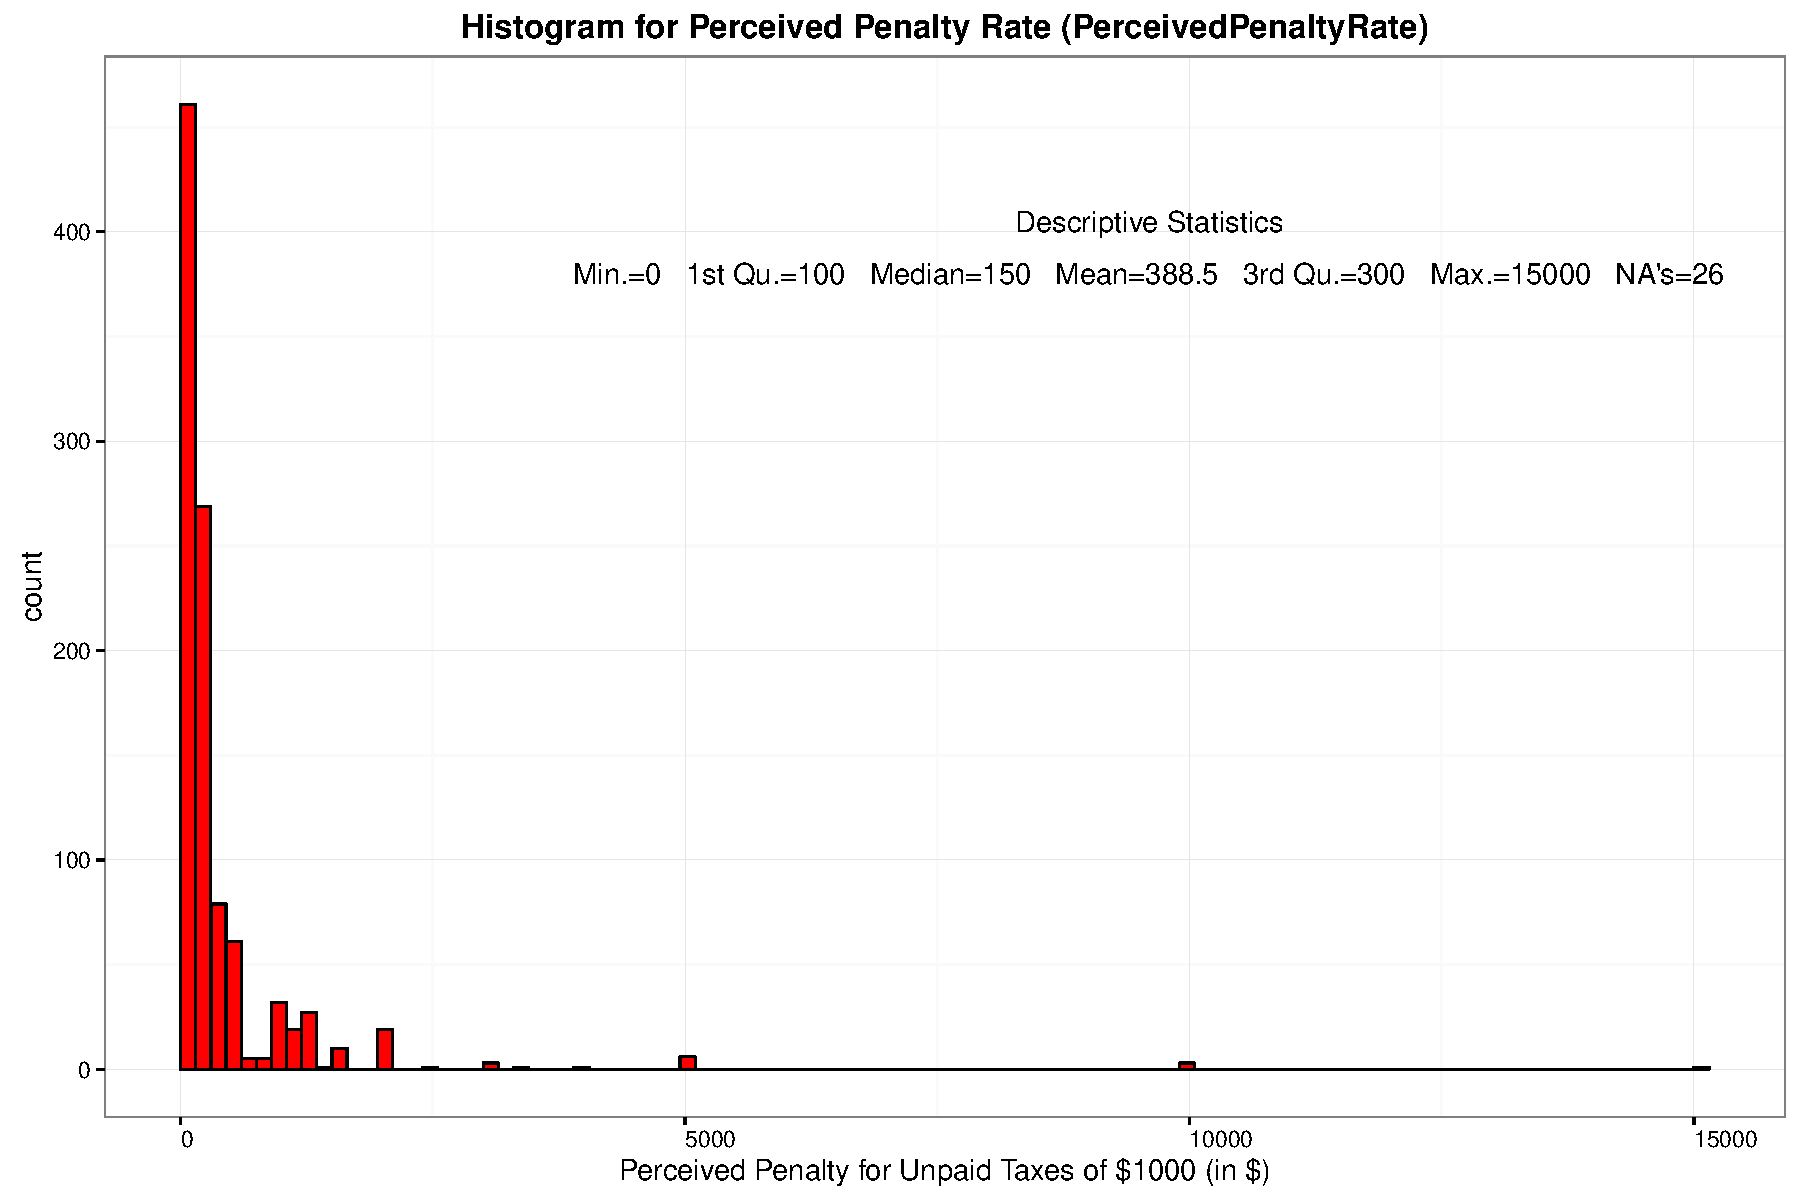
\includegraphics[width = 0.61\textwidth]{HistPerceivedPenaltyRate.pdf}
\caption{Imagine a person was caught underpaying their taxes by \$1000. In addition to having to pay that \$1000, how much of a penalty would they have to pay?}
\label{Fig1}
\end{figure}


\begin{table}[ht]
\centering
\begin{tabular}{rr}
  \hline
 & Penalty-rate \\
&  Perception\\ 
  \hline
  n & 1004 \\ 
  mean & 388.5 \\ 
  sd & 906.8 \\ 
  median & 150.0 \\ 
  min & 0.0 \\ 
  max & 15000.0 \\ 
  range & 15000.0 \\ 
  skew & 8.8 \\ 
  kurtosis & 106.7 \\ 
  se & 28.6 \\ 
   \hline
\end{tabular}
\caption{Descriptive Statistics for Penalty-rate Perception} 
\end{table}


\section{Tax-rate Perception}

\begin{figure}[h!]
\centering
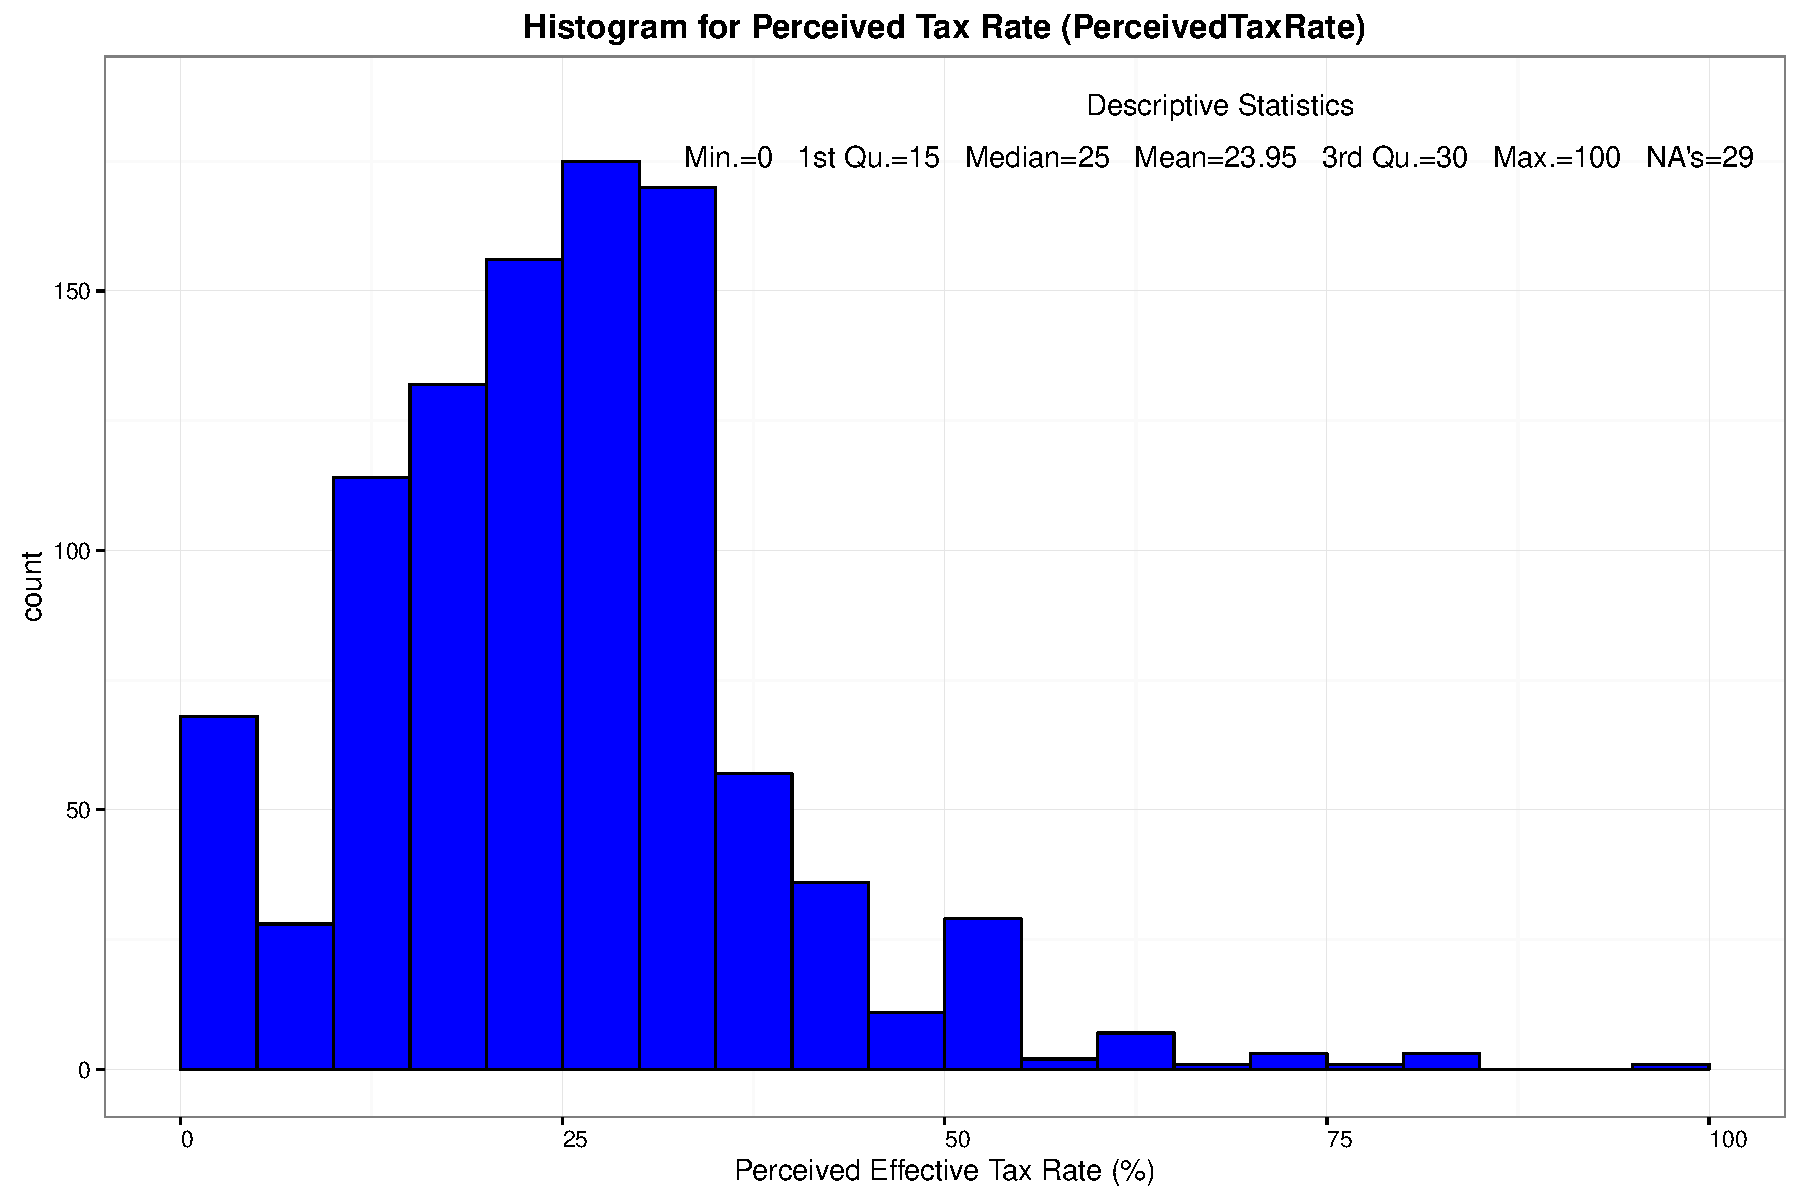
\includegraphics[width = 0.61\textwidth]{HistPerceivedTaxRate.pdf}
\caption{Now let's consider the effective income tax rate.  This is the percent of your income that you owe in taxes to the federal government each year. What do you think your effective income tax rate was this past year?}
\label{Fig2}
\end{figure}
\begin{table}[ht]
\centering
\begin{tabular}{rr}
  \hline
 & Perceived\\ 
& Tax Rate\\
  \hline
  n & 1001 \\ 
  mean & 24.0 \\ 
  sd & 14.3 \\ 
  median & 25.0 \\ 
  min & 0.0 \\ 
  max & 100.0 \\ 
  range & 100.0 \\ 
  skew & 1.5 \\ 
  kurtosis & 6.0 \\ 
  se & 0.5 \\ 
   \hline
\end{tabular}
\caption{Descriptive Statistics for Tax-rate Perception} 
\end{table}

\newpage
\section{Tax Evasion Perception}

\begin{figure}[h!]
\centering
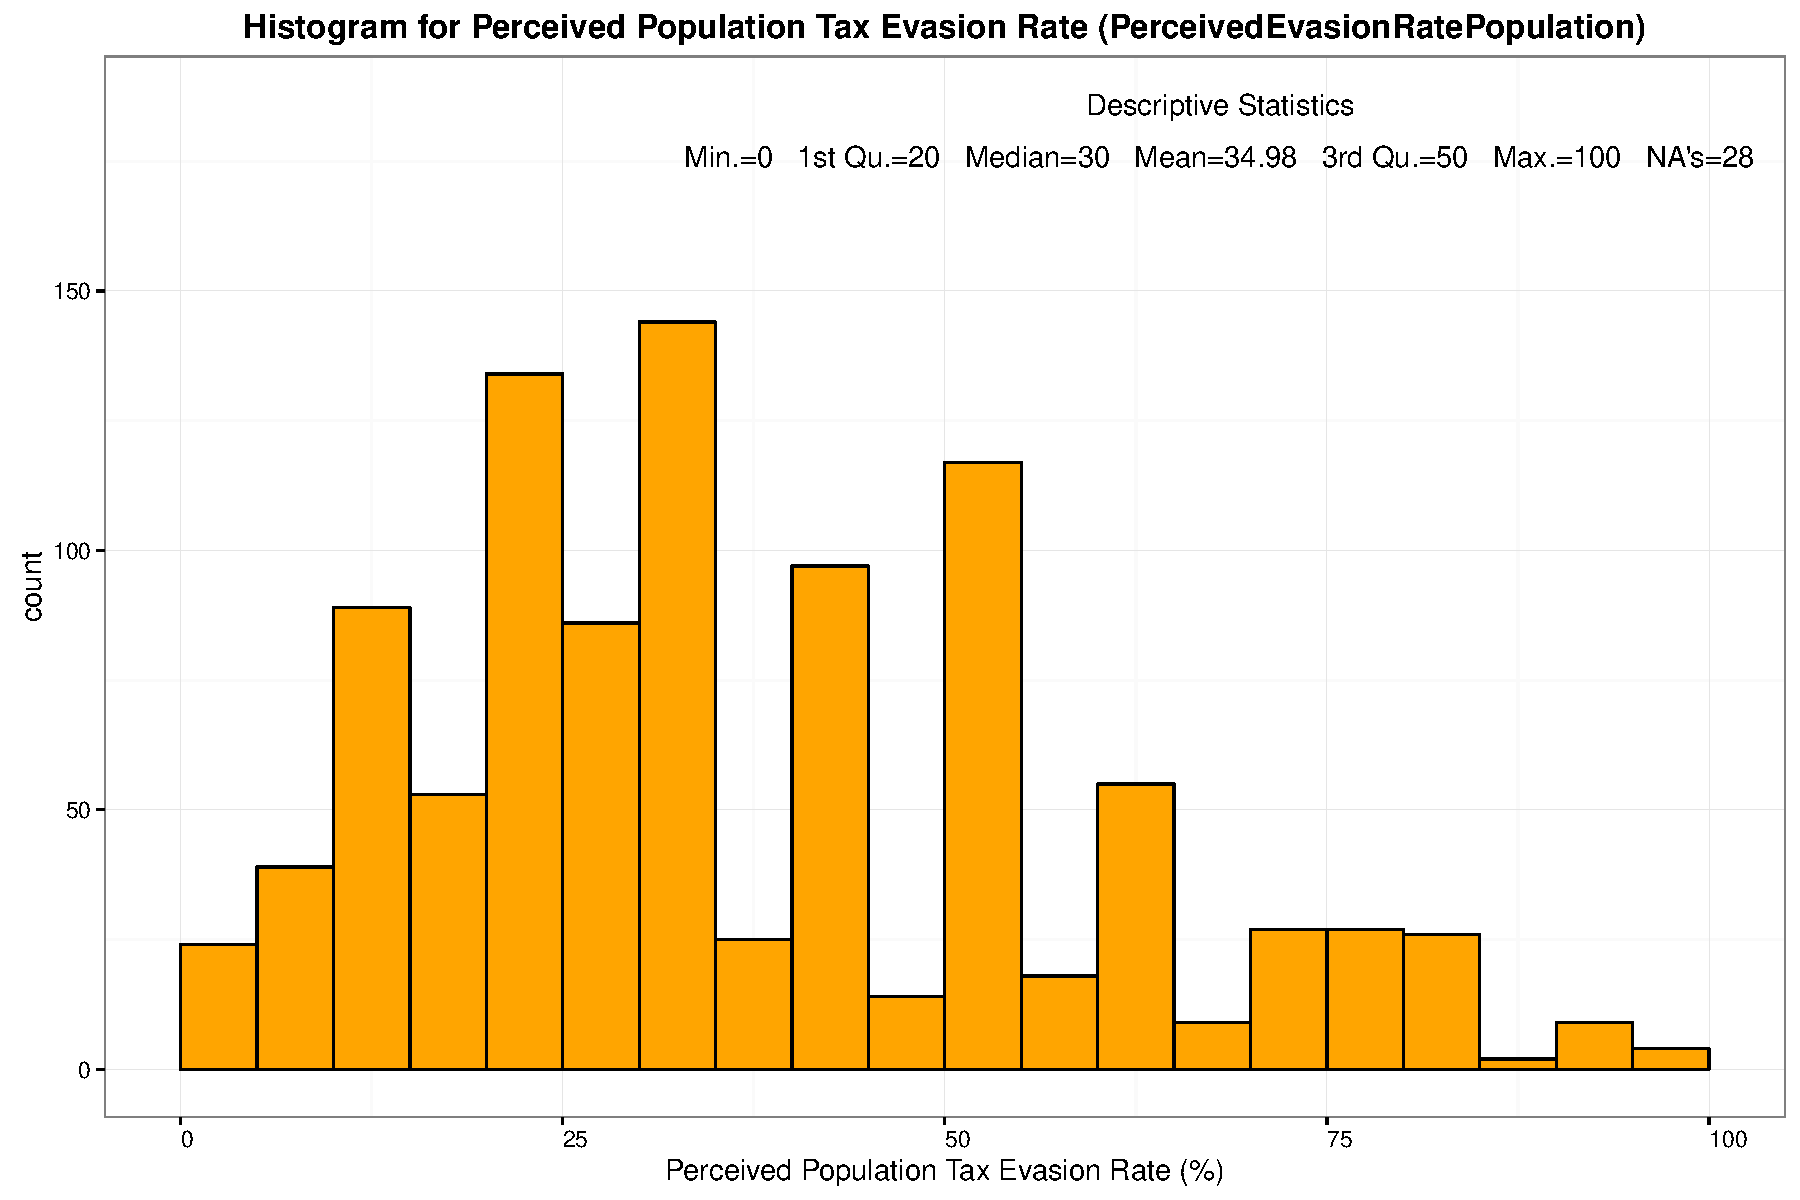
\includegraphics[width = 0.61\textwidth]{HistPerceivedEvasionRatePopulation.pdf}
\caption{In a typical year, out of all taxpayers in the United States, what percent intentionally underreport their taxes?}
\label{Fig3}
\end{figure}


\begin{table}[ht]
\centering
\begin{tabular}{rr}
  \hline
 & Perceived Population\\
 &Tax Evasion Rate (\%) \\ 
  \hline
  n & 1002 \\ 
  mean & 35.0 \\ 
  sd & 21.2 \\ 
  median & 30.0 \\ 
  min & 0.0 \\ 
  max & 100.0 \\ 
  range & 100.0 \\ 
  skew & 0.7 \\ 
  kurtosis & -0.1 \\ 
  se & 0.7 \\ 
   \hline
\end{tabular}
\caption{Descriptive Statistics for Perceived Population Tax Evasion Rate} 
\end{table}


\begin{figure}[h!]
\centering
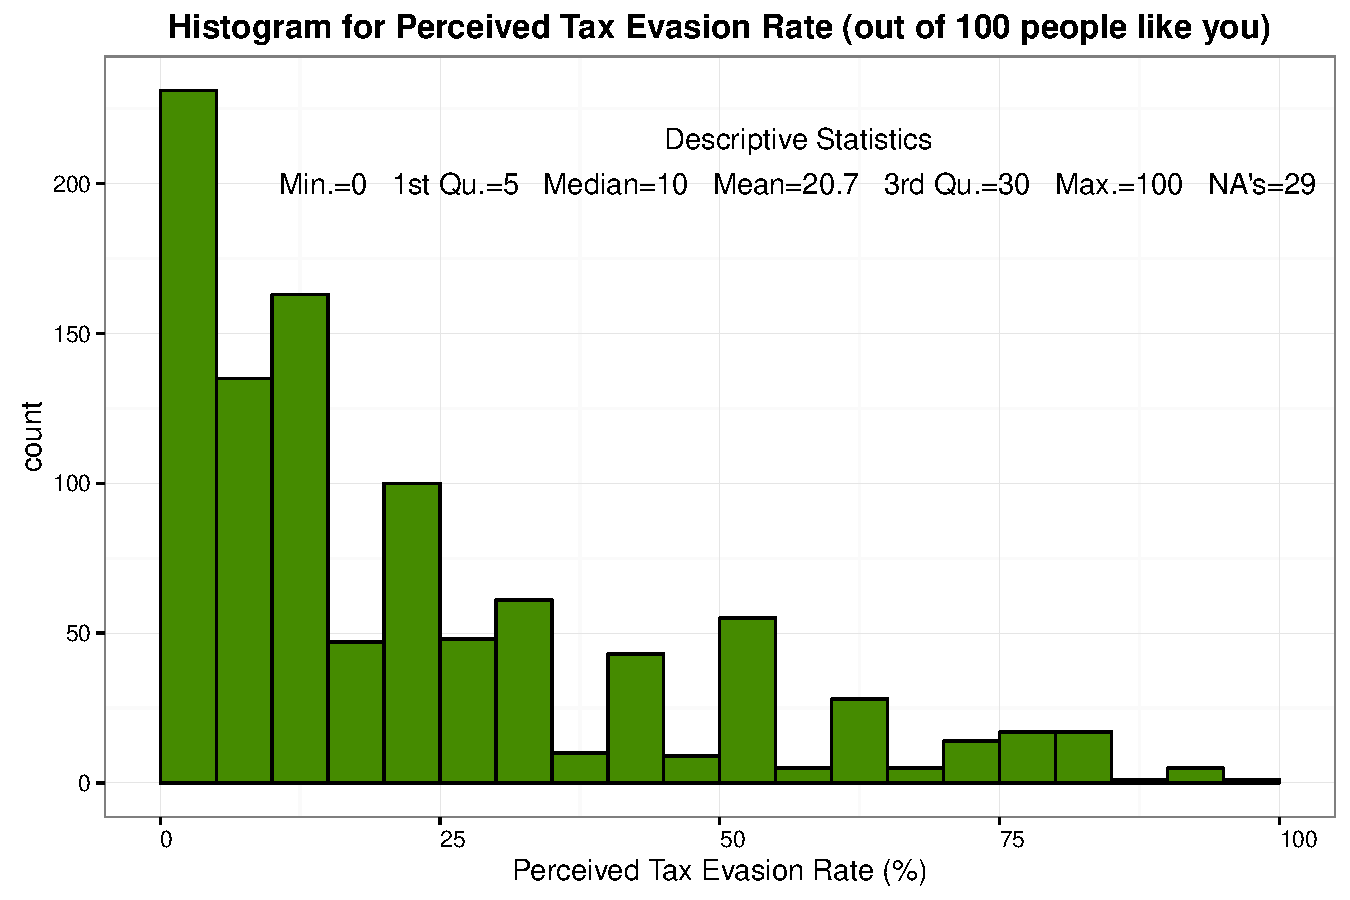
\includegraphics[width = 0.61\textwidth]{HistPerceivedEvasionRate.pdf}
\caption{Now consider people like you. In a typical year, out of 100 people like you, how many intentionally underreport their taxes?}
\label{Fig4}
\end{figure}


\begin{table}[ht]
\centering
\begin{tabular}{rr}
  \hline
 & Perceived Tax\\
& Evasion Rate\\ 
  \hline
  n & 1001 \\ 
  mean & 20.7 \\ 
  sd & 22.4 \\ 
  median & 10.0 \\  
  min & 0.0 \\ 
  max & 100.0 \\ 
  range & 100.0 \\ 
  skew & 1.4 \\ 
  kurtosis & 1.2 \\ 
  se & 0.7 \\ 
   \hline
\end{tabular}
\caption{Descriptive Statistics for Perceived Tax Evasion Rate (out of 100 people like you)} 
\end{table}


\begin{figure}[h!]
\centering
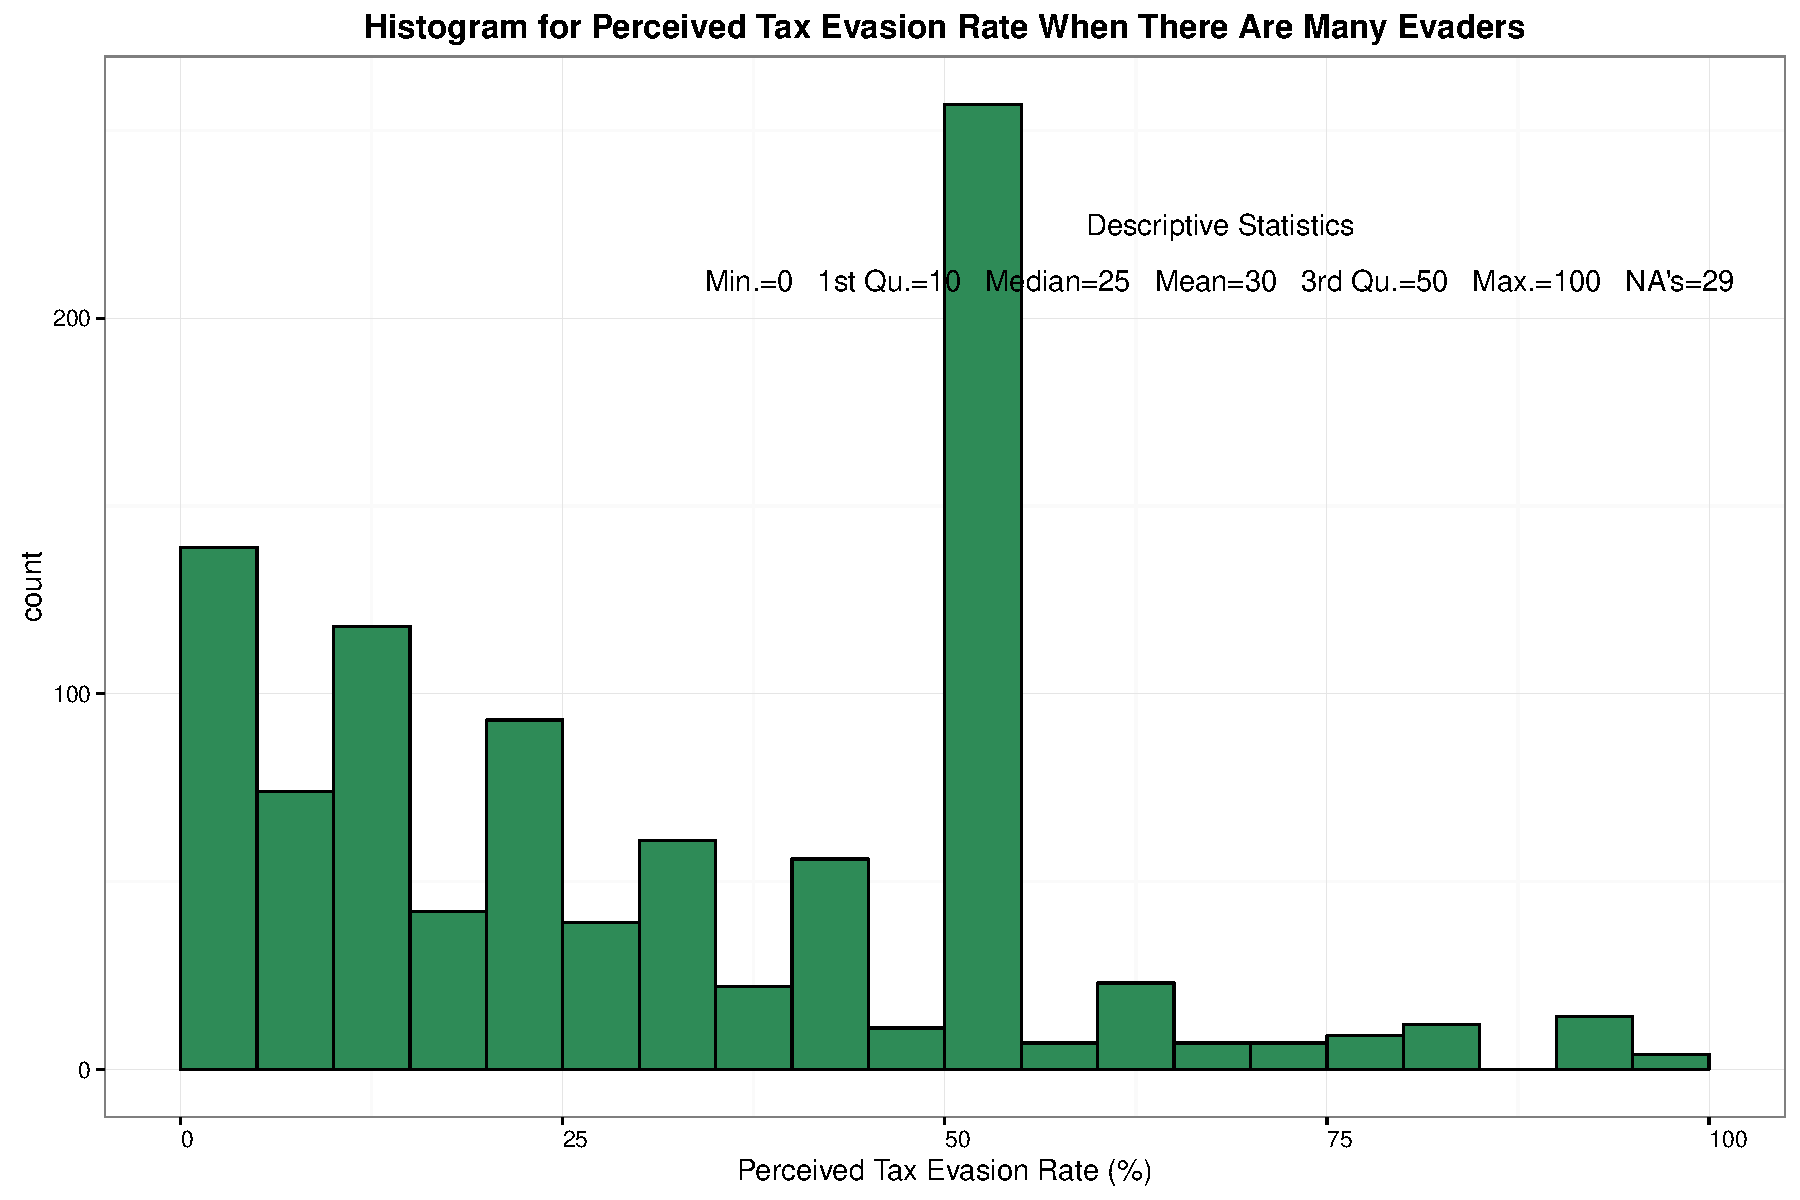
\includegraphics[width = 0.61\textwidth]{HistPerceivedEvasionManyEvaders.pdf}
\caption{Imagine that a widely-disseminated news story comes out that half of all US taxpayers underreport their taxes. Out of 100 people like you, how many would now underreport their taxes?}
\label{Fig5}
\end{figure}


\begin{table}[ht]
\centering
\begin{tabular}{rr}
  \hline
 & Perceived Tax Evasion Rate\\ 
& (When there are many evaders)\\
  \hline
  n & 1001 \\ 
  mean & 30.0 \\ 
  sd & 23.2 \\ 
  median & 25.0 \\  
  min & 0.0 \\ 
  max & 100.0 \\ 
  range & 100.0 \\ 
  skew & 0.5 \\ 
  kurtosis & -0.3 \\ 
  se & 0.7 \\ 
   \hline
\end{tabular}
\caption{Descriptive Statistics for Perceived Tax Evasion Rate (when half of all US taxpayers evade taxes)} 
\end{table}


\clearpage
\section{The Token Questions}

\begin{table}[ht]
\centering
\begin{tabular}{rrrr}
  \hline
 & Q1 & Mean & Q3 \\ 
  \hline
The amount of taxes that I owe & 20.0 & 34.3 & 50.0 \\ 
  The cost to figure out taxes & 5.0 & 13.0 & 20.0 \\ 
  Benefits and public services supported by taxes & 10.0 & 22.4 & 30.0 \\ 
  A moral obligation to report and pay taxes & 15.0 & 30.3 & 40.0 \\ 
   \hline
\end{tabular}
\caption{Imagine that you have 100 tokens. Please allocate 100 tokens to the issues below. 
More tokens means more important.In terms of how you think about taxes and paying your taxes, how 
       important is each of the following?} 
\end{table}

\vspace{18pt}

\begin{table}[ht]
\centering
\begin{tabular}{rrrr}
  \hline
 & Q1 & Mean & Q3 \\ 
  \hline
	Your own thoughts & 40.0 & 54.8 & 70.0 \\ 
  What you hear and know from friends, family, and other close contacts & 10.0 & 22.3 & 30.0 \\ 
  What you hear broadly from the media and other sources & 10.0 & 22.9 & 30.0 \\ 
   \hline
\end{tabular}
\caption{Now let's consider your thoughts on the \underline{fairness of taxes}, and what 
you've seen and heard from those around you.Again, please allocate 100 tokens to the issues below.  
In terms of how fair taxes seem to you, how important is each of the following?} 
\end{table}

\vspace{18pt}

\begin{table}[ht]
\centering
\begin{tabular}{rrrr}
  \hline
 & Q1 & Mean & Q3 \\ 
  \hline
	Your own thoughts & 40.0 & 57.8 & 80.0 \\ 
  What you hear and know from friends, family, and other close contacts & 10.0 & 20.3 & 30.0 \\ 
  What you hear broadly from the media and other sources & 10.0 & 21.9 & 30.0 \\ 
   \hline
\end{tabular}
\caption{Now let's consider your thoughts on the \underline{risk of audits and penalties} for not paying 
one's taxes.  Again, please allocate 100 tokens to the issues below.In terms of how you think about these
risks, how important is each of the following?} 
\end{table}
\end{document}